\documentclass[class=article, crop=false, 12pt]{standalone}
\usepackage[subpreambles=true]{standalone}
\usepackage{../.common/common}


\author{Tony Shing}
%\pretitle{Supplementary}

\topic{T10B (Thermodynamics)}
\title{Maxwell-Boltzmann Distribution}

\version{2025} % leave blank for omitting

\begin{document}

\maketitle


\begin{overview}
    \begin{itemize}
        \item Prerequisite: Probability, extending to continuous random variables
        \item Boltzmann factor
        \item Deriving Maxwell-Boltzmann distribution
    \end{itemize}

\end{overview}


% content begins here
% Section %%%%%%%%%%%%%%%%%%%%%%%%%%%%%%%%%%%%%%%%%%%%%%%%%%%%
\section{Probability Distribution: Discrete \& Continuous}

%%%%%%%%%%%%%%
\subsection{Probabilty Mass Function (PMF)}

For random variables that can be picken from a finite number cases,
we describe them using the \bf{probability mass function} (PMF), $P(x)$,
or most of the time we just call them probabilities.\\

E.g. By throwing 2 dices and sum their values, 
we obtain a list of different probabilities for getting any integer between 2 to 12.

\begin{center}
    \begin{minipage}{0.55\linewidth}
        \centering
        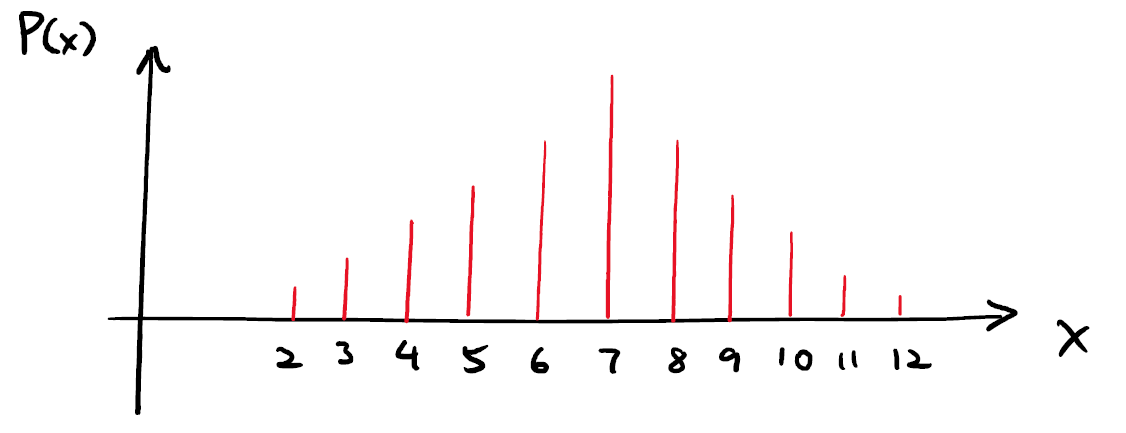
\includegraphics[width=\textwidth]{pmf}
    \end{minipage}
\end{center}

\begin{itemize}
    \item \bf{\ul{Normalization requriement}}:
    The probability of all possible outcomes add up to 1.
    \aleq{
        \sum_{\text{all possible }x_i} P(x_i) = 1
    }

    \item \bf{\ul{Expected value}}: 
    i.e. The weighted average of all outcomes according to the probabilities,
    which is the average value you would get after repeating the process $\infty$ times.
    \aleq{
        \E[x]\quad \defeq \sum_{\text{all possible }x_i} x_i P(x_i)
    }

    \item \bf{\ul{Variance}}:
    It is the average of $(\text{distance})^2$ of all outcomes relative to the expected value.
    Taking square root gives the \bf{standard derivation} (S.D.) = $\sqrt{\text{Variance}}$. 
    \addBentArrow[red]{En}{(-4ex,-2ex)}{\scriptsize Then take average}
    {(0,-1.5ex)}{(-6ex,0.5ex)}
    \addBentArrow[blue]{var}{(4ex,-2ex)}
    {\scriptsize $(x-\E{x})$ = x's distance from the expected value\\[-1ex] \scriptsize Square for taking magnitude only}
    {(0,-1.5ex)}{(17.5ex,-0.5ex)}
    \aleq{
        \Var{x} &\defeq 
        \tkn{En}{\cul[red]{\E}}[\tkn{var}{\cul[blue]{(x-\E{x})^2}}]
    }
    
\end{itemize}

\begin{notation}[Side note:]
    In a special case where there are $N$ different outcomes and every outcome has equal probability to occur,
    \aleq{
        P(x_i) = \frac{1}{N}
    }
    Then the expected value, variance and S.D. will reduce to the formula that we can find in high school textbook.
    \aleq{
        \E{x} &= \sum_{\text{all possible }x_i} x_i P(x_i) = \frac{\sum_i x_i}{N} \ \defeq\ \bar{x} \\[1ex]
        %
        \Var{x} &= \E{(x-\E{x})^2} = \frac{\sum_i (x_i-\E{x})^2}{N} = \frac{\sum_i (x_i-\bar{x})^2}{N} \\[1ex]
        %
        \text{S.D.} = \sqrt{\Var{x}} &= \sqrt{\frac{\sum_i (x_i-\bar{x})^2}{N}}
    }

\end{notation}


%%%%%%%%%%%%%%
\subsection{Probability Density Function (PDF)}

For random variables that can apprear as any value within an interval,
we describe them using the \bf{probability density function} (PDF).

\begin{center}
    \begin{minipage}{0.5\linewidth}
        \centering
        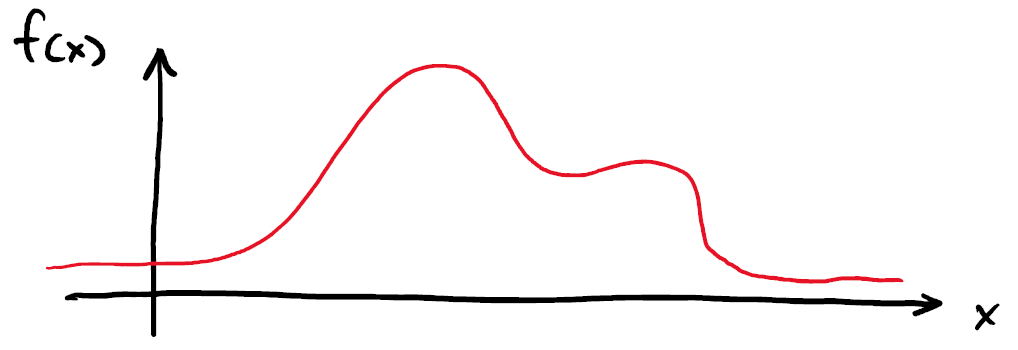
\includegraphics[width=\textwidth]{pdf}
    \end{minipage}
\end{center}


Pay attention here: the output value of the PDF, $f(x)$, 
is NOT the probability of getting $x$. 
This is because there are always infinitely many real number along any interval of real numbers.
\red{The probability of getting an exact number is limited to $0$.}\\

Instead, PDF can only describe the probability of getting a value within an interval $[x_0,x_0+\dd{x}]$.
\aleq{
    P(\tkn{pdf_range}{\cul[green]{x_0<x<x_0+\dd{x}}}) = \tkn{pdf_f}{\cul[blue]{f(x)}}\tkn{pdf_dx}{\cul[red]{\dd{x}}}
}
\addArrow[green]{pdf_range}{(0,-2ex)}{\scriptsize Prob. inside the interval}{(0,-1ex)}
\addArrow[blue]{pdf_f}{(0,-3ex)}{\scriptsize height}{(0,-1.5ex)}
\addArrow[red]{pdf_dx}{(3ex,-2ex)}{\scriptsize width}{(0,-1ex)}


\begin{center}
    \begin{minipage}{0.6\linewidth}
        \centering
        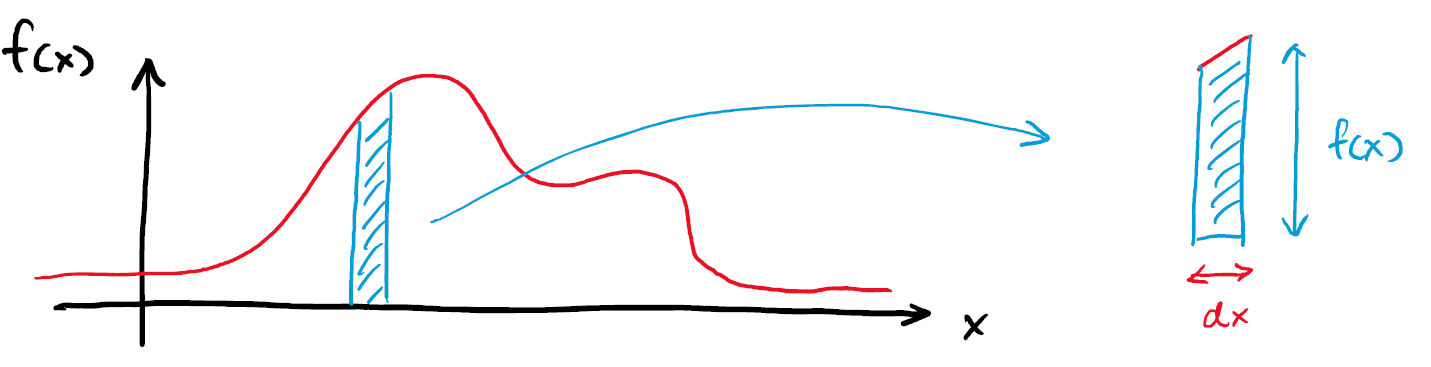
\includegraphics[width=\textwidth]{pdf_area}
    \end{minipage}
\end{center}

As interpreted, the probability is represented by the \cul[red]{area under curve $f(x)\dd{x}$},
not the height $f(x)$. This is also why it is named "density" function - 
the probability per "length" of $x$.

\newpage
The formula for PMF (discrete cases) can be extended to PDF (continuous cases).
\begin{itemize}
    \item \bf{\ul{Normalization requriement}}: 
    The probability of all possible cases add up to 1.
    From the condition for PMF, we can extend the sum to integral for PDF.
    \aleq{
        \sum_{\text{all possible }x_i} P(x_i) = 1 
        \qquad\Rightarrow\qquad 
        \int_{-\infty}^\infty f(x) \dd{x} = 1
    }

    \item \bf{\ul{Expected value}}: 
    The weighted average of all outcomes according to the probabilities.
    Can be understand by the weighted sum interpretation of integration.
    \aleq{
        \E{x}\quad \defeq \sum_{\text{all possible }x_i} x_i P(x_i) 
        \qquad\Rightarrow\qquad
        \E{x} \ \defeq\  \int_{-\infty}^{\infty} xf(x) \dd{x}
    }

    \item \bf{\ul{Variance}}:
    Same as in the discrete case, it is the average of $(\text{distance})^2$ of all outcomes relative to the expected value.
    \aleq{
        \Var{x}\ \defeq\ \E{(x-\E{x})^2} 
        \qquad\Rightarrow\qquad
        \Var{x} \ \defeq\  \int_{-\infty}^{\infty} (x-\E{x})^2 f(x) \dd{x}
    }
    Taking square root gives the standard derivation (S.D.) = $\sqrt{\Var{x}}$. 

\end{itemize}


\linesep
% Section %%%%%%%%%%%%%%%%%%%%%%%%%%%%%%%%%%%%%%%%%%%%%%%%%%%%
\section{Boltzmann Distribution}

%%%%%%%%%%%%%%%%%
\subsection{Thermal Fluctuation}

In thermodynamics, every state parameter is a statistical property - 
a state being labeled with parameter $x=x_0$ only means the \cul[red]{expected value of observing $x$ is $x_0$}.
Its actual value can random fluctuate, 
different in value from time to time.\\

For example, in the 2-boxes system with 1000 balls, 
the macrostates are described by one state parameter $N_R=$ the number of balls in the right box. 
Because the balls are always free to move between the boxes, 
$N_R$ must fluctuate, even when it has reached the maximum entropy state 500L-500R. 
\begin{itemize}
    \item
    One of the ball may temporarily move from the left box to the right box.
    The system's state change to 499L-501R. 

    \item After some time, another ball moves from the right box to the left box.
    The system's state returns to 500L-500R.
\end{itemize}

\insertFig{moving ball in and out}

Because of this randomness, 
we expect that measurement to any parameter $x$ will form some probabiilty distribution centered around its expected value $x=x_0$.
\begin{center}
    \red{When the system is in the macrostate $x=x_0$,
    what is the probability to observe $x$ to be $x_0 + \Delta x$?}
\end{center}

Recall that the probability of observing a macrostate with parameter $x$ 
is proportional to the number of microstates (i.e. multiplicity) it corresponds to,
\aleq{
    P\qty(x=x_0) 
    \ &\propto\ %\frac{\qty(\mstack{\text{\# of microstates that}\\\text{leads to observing }x=0})}{\qty(\text{Total \# of microstates})}
    \mstack{\text{\# of microstates that}\\\text{leads to observing }x=x_0}\\
    &= \inv{Z}W(x=x_0) = \inv{Z}e^{\frac{S(x=x_0)}{k}}
}

where $Z$ is some constant for normalization (because probability should add up to $1$).
It can be calculated as
\aleq{
    Z = 
    \bcase{
        \sum_{\substack{\text{all possible}\\x_i}}W(x_i) = x_i
    }
}

\begin{notation}[Side note:]
    Recall the statement of Clausius theorem - 
    entropy of a closed system must either be a constant 
    or increase along any process.
    However this is only true for the expected value. 
    \aleq{
        \Delta S \geq 0 \quad\xRightarrow{\text{More accurately}}\quad \Delta S_\red{\text{avg.}} \geq 0
    }

    Irreversibility exists only because systems tend to evolve from 
    macrostates of low multiplicity to high multiplicity.
    The reverse is allowed to happen,
    although at a much lower chance.\\

    The fluctuation in multiplicity is most likely observed after the system has reached its maximum entropy state - 
    because any fluctuation will cause the system evolves into a lower multiplicity state.
    Afte some time  multiplicity increases again due to probability.
\end{notation}







And multiplicity is related to the entropy of the macrostate. 
So if we know the function form of multiplicity or entropy related to the parameter, i.e. $W(x)$ or $S(x)$,
we can tell the probability of observing a particular value of $x$.
\aleq{
    P\qty(x=x_0) 
    \ =\ \frac{e^{\frac{S(x_0)}{k}}}{Z}
    \qquad\text{where}\qquad Z = \sum_{\substack{\text{all possible}\\x_0}}e^{\frac{S(x_0)}{k}} 
}

In particular, if the system is at its maximum entropy state when $x=x^\ast$,
we can relate the fluctuation in entropy $\Delta S$ can be related to 
the fluctuation of the state parameter $\Delta x$ by Taylor series expansion:
\aleq{
   S(x^\ast+\Delta x) &= S(x^\ast) + \Delta S\\ 
   &= S(x^\ast) + \pdvv{S}{x}\eval_{x=x^\ast} (\Delta x) + \half \pdvv[2]{S}{x}\eval_{x=x^\ast} (\Delta x)^2 + \cdots
}


Suppose the system has a state parameter $x$ 
(E.g. In the 2-boxes model, we have $x$ = number of balls in the right box).
What is the probability to observe it fluctuates by a magnitude $\Delta x$?\\



In general, we can express the entropy $S$ of a system as a function of another state parameter $x$ 




%%%%%%%%%%%%%%
\subsection{Boltzmann Distribution}

The fluctuation for internal energy is a bit more interesting - 
because energy of a closed system must be a constant, 
there shall not be fluctuation for the \ul{total internal energy}.
However, we can consider the fluctuation of internal energy on individual objects in the system.


A direct consequence of entropy fluctuation is that objects in a closed system are allowed to exchange energy
(as long as total energy conserves).



Now we can apply the fluctuation 
However one thing very different between energy and other state parameters is that -
energy must conserve in any scenario. 






In the simplest 2-boxes model, without energy consideration,
we used $x=n_L=$ number of balls in the left box as the state parameter. 

when two such model is put together,
total multiplicity is just a 

When x=nL, 
nL can take whatever value, 

energy is a conserved quantity
if one object has high energy then the other must have low energy

Multiplicity under Energy Constraint



Recall that in the 2-boxes system with energy difference,
the multiplicity of the system is a function to internal energy.
If the system is closed, 
i.e. its internal energy is constant because it is not in thermal contact with anything, 
then neither its multiplicity or entropy can vary.

\insertFig{bar chart S}

\bf{But in reality, the only closed system is the whole universe}
because 100\% heat insulation from heat radiation does not exist.
Every object in the universe is constantly under thermal contact with other objects - 
sometimes you may observe its internal energy to be some value $U_1$,
and sometimes you may observe it to be another value $U_2$.

\begin{center}
    \red{What is the probability to observe that the object carry internal energy $U_i$?}
\end{center}




Previously, we have only dealt with closed system - 
any objects that involve in heat exchange are considered as part of the system.
\\

\iffalse
A "feature" of closed systems is that, 
once the system has reached the maximum entropy state,
there will be no more thermal interactions -
the system is fixed at this state FOREVER.\\
(P.S. The maximum entropy state of the universe is called "Heat death".)

\insertFig{heat exchange of two object -> eqm forever}


Anyway we are unable to consider every object in the universe.
To correctly model objects' thermal behaviors,
they should be treated as open systems - 
the internal energy on the object is no longer a fixed value because of heat fluctuation,
the ,
but can lie in a range of values.





if we know the probability distribution of $U$, 
i.e. how frequent is this object found to have energy $U$, 
then we can calculate the total multiplicity as the expected value under this distribution:
\aleq{
    W_\text{obj} &= \sum_{\substack{\text{all possible}\\U_i}} 
    \qty(\mstack{\text{Multiplicity when}\\\text{the object}\\\text{has energy } U_i}) \times 
    \qty(\mstack{\text{Probability of}\\\text{the object}\\\text{having energy } U_i})\\[0.5em]
    %
    &=  
    \begin{cases}
        \displaystyle
        \sum_{\substack{\text{all possible}\\U_i}} W(U_i)P(U_i) 
        &\text{(if }U\text{ can only have discrete values)}\\[2em]
        %
        \displaystyle
        \int_{\substack{\text{possible}\\\text{range}\\\text{of }U}} W(U) P(U)\dd{U}
        &\text{(if }U\text{ can be a continuous range of values)}
    \end{cases}
}

\vskip 1ex
How do you find $P(U)$?
\fi

%%%%%%%%%%%%%%
\subsection{The Boltzmann Factor}

We model the object as \cul[red]{thermally} contacting with a HUGE heat bath (i.e. the universe),
where the only form of energy exchange is by heat transfer.

\insertFig{heat bath contact}

We require the following assumptions: 
\begin{enumerate}
    \item The heat bath is so HUGE that any energy exchange has no effect on it.
    Its state parameters (e.g. temperature, entropy,...) remains constant all the time. 

    \item The total energy of the object + heat bath is conserved.
    \aleq{
        U_\text{total} = U_\text{bath} + U_\text{obj} = \text{const.}
    }
    \item Energy carried by the heat bath is much greater than the energy carried by the object. i.e.
    \aleq{
        U_\text{bath} \gg U_\text{obj}
    }
\end{enumerate}

Let the entropy of the heat bath be $S_\text{bath}$,
which must be some function to its internal energy $U_\text{bath}$ 
(although we do not know what this function is).
We can make a Taylor expansion by
\aleq{
    S_\text{bath} &= S_\text{bath}(U_\text{bath}) \\
    %
    &= S_\text{bath}(\red{U_\text{total} - U_\text{obj}})\\[1ex]
    %
    &\approx S_\text{bath}(U_\text{total}) - \dvv{S_\text{bath}}{U}\eval_{U=U_\text{total}}\cdot U_\text{obj}\\
    %
    &= S_\text{bath}(U_\text{total}) - \frac{U_\text{obj}}{T_\text{bath}}
}

The total multiplicity of the \{heat bath + object\} is thus
\aleq{
    S_\text{total} &= S_\text{bath}+ S_\text{obj}\\
    %
    W_\text{total} &= e^\frac{S_\text{bath}+ S_\text{obj}}{k} \\
    %
    &\approx e^\frac{S_\text{bath}(U_\text{total}) -  \frac{U_\text{obj}}{T_\text{bath}}}{k} \cdot e^\frac{S_\text{obj}}{k}\\
    %
    &= e^\frac{S_\text{bath}(U_\text{total})}{k} \cdot e^{-\frac{U_\text{obj}}{kT_\text{bath}}} \cdot e^\frac{S_\text{obj}}{k}\\
    %
    &= \tkn{W_const}{\cul[red]{e^\frac{S_\text{bath}(U_\text{total})}{k}}} \cdot e^{-\frac{U_\text{obj}}{kT_\text{bath}}} \cdot \tkn{W_obj}{\cul[blue]{W_\text{obj}}}
}
\addArrow[red]{W_const}{(-3ex,-2ex)}
{\scriptsize $U_\text{total}$ is a constant\\[-1ex]\scriptsize so this term is just a constant}
{(0,-1ex)}{(0,-1.5ex)}
\addArrow[blue]{W_obj}{(3ex,-2ex)}
{\scriptsize Multiplicity of the object\\[-1ex]\scriptsize is some function of $U_\text{obj}$}
{(0,-1.5ex)}{(0,-1.5ex)}

\vskip 1em
Now the total multiplicity is expressed purely a function of $U_\text{obj}$.
This is the total multiplicity (i.e. number of microstates) when the object has a particular value of internal energy $U_\text{obj}$ 
with the heat bath maintained at temperature $T_\text{bath}$:
\aleq{
    W_\text{total}(U_\text{obj}) = \qty(\text{const.})\cdot e^{-\frac{U_\text{obj}}{kT_\text{bath}}} \cdot W_\text{obj}\qty(U_\text{obj})
}

To find the probability which the object has a particular value of internal energy $U_\text{obj}$,
we simply divide it by the total multiplicity (total number of microstates),
which is summed from all possible $U_\text{obj}$.
\aleq{
    P(U_\text{obj}) = \frac{W_\text{total}(U_\text{obj})}{\displaystyle \sum_{\substack{\text{all possible}\\U_\text{obj}}}W_\text{total}(U_\text{obj})}
}

But the thing we are actually interested in is the probability to find the object having centain value of internal energy.
Recall the relation between multiplicity and probability:
\aleq{
    W(U) = 
}



Let the entropy-energy relation of the heat bath and the object be some functions 
(which we may or may not know its formula),
\aleq{
    \qquad,\qquad
    S_\text{obj} = S_\text{obj}(U_\text{obj}) 
}




%%%%%%%%%%%%%%
\subsection{Example: System with Discrete Energy States}





\linesep
% Section %%%%%%%%%%%%%%%%%%%%%%%%%%%%%%%%%%%%%%%%%%%%%%%%%%%%
\section{Density of State of Ideal Gas}



The most important application of the above ideas is to find the
energy-probability relation for states in ideal gas,
when heat exchange is allowed.\\

i.e. States with which energy are most probable to be found,
given that it is at temperature $T$?\\

Since energy of ideal gas can be any real number,
we first need to adapt the formula from last section for continuous distribution.
\aleq{
    \sum_{\substack{\text{all possible}\\U}} e^{-\frac{U}{kT}} W(U) 
    \qquad\rightarrow\qquad
    \int_0^\infty e^{-\frac{U}{kT}}W(U) \dd{U}
}W

What is the $W(U)$ for ideal gas?



%%%%%%%%%%%%%%
\subsection{Entropy of Ideal Gas}


%%%%%%%%%%%%%%
\subsection{Average Speed of Ideal Gas}

In textbooks you can find 2 different formulas 
related to the average speed about ideal gas. 
How are they derived?

\begin{enumerate}
    \item \bf{\ul{Average Speed}} = Expected value to $\abs{v}$, i.e. $\E(\abs{v})$.
    \aleq{
        \E(\abs{v}) &= \int^\infty_0 \abs{v} \cdot P(\abs{v}) \dd{\abs{v}}\\
        %
        &= \int^\infty_0 \abs{v} \cdot \sqrt{\frac{2m^3}{\pi k^2 T^3}} \abs{v}^2 e^{-\frac{m\abs{v}^2}{2kT}} \dd{\abs{v}}\\
        %
        &= \sqrt{\frac{2m^3}{\pi k^2 T^3}} \qty(\frac{2kT}{m})^2 \int^\infty_0 \qty(\sqrt{\frac{m}{2kT}}v)^3 e^{-\qty(\sqrt{\frac{m}{2kT}}v)^2} \dd{\qty(\sqrt{\frac{m}{2kT}}v)}\\
        %
        &= \sqrt{\frac{32kT}{\pi m}} \int^\infty_0 x^3 e^{-x^2} \dd{x} \\
        %
        &= \sqrt{\frac{32kT}{\pi m}} \cdot \half\\
        %
        &= \sqrt{\frac{8kT}{\pi m}}  \defeq  v_\text{avg}
    }

    \item \bf{\ul{Root Mean Square Speed}} = $\sqrt{\text{Expected value to } \abs{v}^2}$, i.e. $\sqrt{\E(\abs{v}^2)}$.
    \aleq{
        \E(\abs{v}^2) &= \int^\infty_0 \abs{v}^2 \cdot P(\abs{v}) \dd{\abs{v}}\\
        %
        &= \int^\infty_0 \abs{v}^2 \cdot \sqrt{\frac{2m^3}{\pi k^2 T^3}} \abs{v}^2 e^{-\frac{m\abs{v}^2}{2kT}} \dd{\abs{v}}\\
        %
        &= \sqrt{\frac{2m^3}{\pi k^2 T^3}} \qty(\frac{2kT}{m})^3 \int^\infty_0 \qty(\sqrt{\frac{m}{2kT}}v)^3 e^{-\qty(\sqrt{\frac{m}{2kT}}v)^2} \dd{\qty(\sqrt{\frac{m}{2kT}}v)}\\
        %
        &= \sqrt{\frac{64k^2T^2}{\pi m^2}} \int^\infty_0 x^4 e^{-x^2} \dd{x} \\
        %
        &= \sqrt{\frac{64k^2T^2}{\pi m^2}}\cdot \frac{3\sqrt{\pi}}{8} \\
        %
        &= \frac{3kT}{m}\\
        %
        \sqrt{\E(\abs{v}^2)} &= \sqrt{\frac{3kT}{m}}  \defeq  v_\text{rms}
    }
\end{enumerate}

\bf{\ul{Note}}: Because the average KE
(which is something we can measure)
is calculated as 
\aleq{
    \text{Avg. KE} &= \E\qty(\half m\abs{v}^2) \\
    &= \half m \E(\abs{v}^2)\\
    &= \half m v_\text{rms}^2 
}

The root mean square speed is way more useful than the average speed.

%%%
\theend
\end{document}